%%%%%%%%%%%%%%%%%%%%%%%%%%%%%%%%%%%%%%%%%%%%%%%%%%%%%%%%%%%%%%%%%%%%%%%%%%%%%
%%%
%%% File: thesis.tex, version 1.9, May 2016
%%%
%%% =============================================
%%% This file contains a template that can be used with the package
%%% cs.sty and LaTeX2e to produce a thesis that meets the requirements
%%% of the Computer Science Department from the Technical University of Cluj-Napoca
%%%%%%%%%%%%%%%%%%%%%%%%%%%%%%%%%%%%%%%%%%%%%%%%%%%%%%%%%%%%%%%%%%%%%%%%%%%%%

\documentclass[12pt,a4paper,twoside]{report}         
\usepackage{cs}              
\usepackage{times}
\usepackage{graphicx}
\usepackage{latexsym}
\usepackage{amsmath,amsbsy}
\usepackage{amssymb}
\usepackage[matrix,arrow]{xy}
\usepackage[T1]{fontenc}
\usepackage{ae,aecompl}
\usepackage{romanian} %definitii pentru diacritice; 
\usepackage{amstext}
\usepackage{graphics}
\usepackage[T1]{fontenc}
\usepackage{ae,aecompl}
\usepackage{algorithm}
%\usepackage{algorithmic}
\usepackage{color}
\usepackage{color}

% \mastersthesis
\diplomathesis
% \leftchapter
\centerchapter
% \rightchapter
\singlespace
% \oneandhalfspace
% \doublespace

\renewcommand{\thesisauthor}{Prenume NUME}    %% Your name.
\renewcommand{\thesismonth}{Iunie}     %% Your month of graduation.
\renewcommand{\thesisyear}{2019}      %% Your year of graduation.
\renewcommand{\thesistitle}{TITLUL LUCR'ARII DE LICEN'T'A} % Title
\renewcommand{\thesissupervisor}{titlul 'stiin'tific Prenume NUME}
\newcommand{\department}{FACULTATEA DE AUTOMATIC'A 'SI CALCULATOARE\\
DEPARTAMENTUL CALCULATOARE}
\newcommand{\thesis}{LUCRARE DE LICEN'T'A}
\newcommand{\uline}[1]{\rule[0pt]{#1}{0.4pt}}
%\renewcommand{\thesisdedication}{P'arin'tilor mei}
\newcommand{\utcnlogo}{
\includegraphics[width=15cm]{img/utcn.jpg}}

\begin{document}
%\frontmatter
%\pagestyle{headings}

\newenvironment{definition}[1][Defini'tie.]{\begin{trivlist}
\item[\hskip \labelsep {\bfseries #1}]}{\end{trivlist}}



%\thesistitle                    %% Generate the title page.
%\authordeclarationpage                %% Generate the declaration page.


\begin{center}
%
\includegraphics[width=15cm]{img/tucn.jpg}  
\utcnlogo

{\bf \department}

\vspace{4cm}

{\bf \thesistitle} %LICENSE THESIS TITLE}

\vspace{1.5cm}

\thesis

\vspace{6cm}

Absolvent: {\bf \thesisauthor} 

Conduc'ator 'stiin'tific: {\bf \thesissupervisor}

\vspace{3cm}
{\bf \thesisyear}
\end{center}

\thispagestyle{empty}
\newpage

\begin{center}
\utcnlogo

{\bf \department}
\end{center}
\vspace{0.5cm}

%\begin{small}
\begin{tabular}{p{7cm}p{8cm}}
 %\hspace{-1cm}& VIZAT,\\
 \hspace{-1cm}DECAN, & DIRECTOR DEPARTAMENT,\\
\hspace{-1cm}{\bf Prof. dr. ing. Liviu MICLEA} & {\bf Prof. dr. ing. Rodica POTOLEA}\\  
\end{tabular}
 
\vspace{2cm}

\begin{center}
Absolvent: {\bf \thesisauthor}

\vspace{1cm}

{\bf \thesistitle}
\end{center}

\vspace{1cm}

\begin{enumerate}
 \item {\bf Enun'tul temei:} {\it Scurt'a descriere a temei lucr'arii de licen't'a 'si datele ini'tiale}
\item {\bf Con'tinutul lucr'arii:} {\it (enumerarea p'ar'tilor componente) Exemplu: Pagina de prezentare, aprecierile coordonatorului de lucrare, titlul capitolului 1, titlul capitolului 2, titlul capitolului n, bibliografie, anexe.}
\item {\bf Locul document'arii:} {\it Exemplu}: Universitatea Tehnic'a din Cluj-Napoca, Departamentul Calculatoare
\item {\bf Consultan'ti:}
\item {\bf Data emiterii temei:} 1 Noiembrie 2018
\item {\bf Data pred'arii:} 8 iulie 2019 {\it (se va completa data pred'arii)}
  \end{enumerate}
\vspace{1.2cm}

\hspace{6cm} Absolvent: \uline{6cm} 

\vspace{0.5cm}
\hspace{6cm} Coordonator 'stiin'tific: \uline{5cm} 
%\end{small}

\thispagestyle{empty}

\newpage

\begin{center}
\utcnlogo

{\bf \department}
\end{center}

\vspace{0.5cm}

\begin{center}
{\bf
Declara'tie pe proprie r'aspundere privind\\ 
autenticitatea lucr'arii de licen't'a}
\end{center}
\vspace{1cm}



Subsemnatul(a) \\
\uline{14.8cm}, 
legitimat('a) cu \uline{4cm} seria \uline{3cm} nr. \uline{4cm}\\
CNP \uline{9cm}, autorul lucr'arii \uline{2.8cm}\\
\uline{16cm}\\
\uline{16cm}\\
elaborat'a 'in vederea sus'tinerii examenului de finalizare a studiilor de licen't'a la Facultatea de Automatic'a 'si Calculatoare, Specializarea \uline{7cm} din cadrul Universit'a'tii Tehnice din Cluj-Napoca, sesiunea \uline{4cm} a anului universitar \uline{3cm}, declar pe proprie r'aspundere, c'a aceast'a lucrare este rezultatul propriei activit'a'ti intelectuale, pe baza cercet'arilor mele 'si pe baza informa'tiilor ob'tinute din surse care au fost citate, 'in textul lucr'arii 'si 'in bibliografie.

Declar, c'a aceast'a lucrare nu con'tine por'tiuni plagiate, iar sursele bibliografice au fost folosite cu respectarea legisla'tiei rom\ia ne 'si a conven'tiilor interna'tionale privind drepturile de autor.

Declar, de asemenea, c'a aceast'a lucrare nu a mai fost prezentat'a 'in fa'ta unei alte comisii de examen de licen't'a.

'In cazul constat'arii ulterioare a unor declara'tii false, voi suporta sanc'tiunile administrative, respectiv, \emph{anularea examenului de licen't'a}.

\vspace{1.5cm}

Data \hspace{8cm} Nume, Prenume

\vspace{0.5cm}

\uline{3cm} \hspace{5cm} \uline{5cm}

\vspace{1cm}
\hspace{9.4cm}Semn'atura

\thispagestyle{empty}

\newpage

%\clearpage 
%\newpage

%\begin{comment}
{\color{red}{\bf De citit 'inainte} (aceast'a pagin'a se va elimina din versiunea final'a)}:
\begin{enumerate}
 \item Cele trei pagini anterioare (foaie de cap'at, foaie sumar, declara'tie) se vor lista pe foi separate (nu fa't'a-verso), fiind incluse 'in lucrarea listat'a. 
 Foaia de sumar (a doua) necesit'a semn'atura absolventului, respectiv a coordonatorului.
 Pe declara'tie se trece data c\ia nd se pred'a lucrarea la secretarii de comisie.
 \item Pe foaia de cap'at, se va trece corect titulatura cadrului didactic 'indrum'ator, 'in englez'a (consulta'ti pagina de unde a'ti desc'arcat acest document pentru lista cadrelor didactice cu titulaturile lor).
 \item Documentul curent {\bf nu} a fost creat 'in MS Office. E posibil sa fie mici diferen'te de formatare. 
\item Cuprinsul 'incepe pe pagina nou'a, impar'a (dac'a se face listare fa't'a-verso), prima pagin'a din capitolul Introducere tot a'sa, fiind numerotat'a cu 1. % Pentru actualizarea cuprinsului, click dreapta pe cuprins (zona cuprinsului va apare cu gri), Update field-$>$Update entire table.
\item Vizualiza'ti (recomandabil 'si 'in timpul edit'arii) acest document % după ce activaţi vizualizarea simbolurilor ascunse de formatare (apăsaţi simbolul  din Home/Paragraph).
\item Fiecare capitol 'incepe pe pagin'a nou'a. % datorită simbolului ascuns Section Break (Next Page) care este deja introdus la capitolul precedent. Dacă ştergeţi din greşeală simbolul, se reintroduce (Page Layout -> Breaks).
\item Folosi'ti stilurile predefinite (Headings, Figure, Table, Normal, etc.)
\item Marginile la pagini nu se modific'a.
\item Respecta'ti restul instruc'tiunilor din fiecare capitol.
\end{enumerate}
\thispagestyle{empty} 
%\end{comment}

\pagenumbering{roman}
\setcounter{page}{1}

\newpage

\tableofcontents

\newpage

%\listoftables
%\listoffigures

\pagenumbering{arabic}
\setcounter{page}{1}

\chapter{Introducere - Contextul proiectului}
\pagestyle{headings}

Titlul capitolului se bazeaz'a pe Heading 1 style, numerotat cu o cifra (x. Nume capitol), font Times New Roman de 14, Bold.

Ce se scrie aici:

\begin{itemize}
 \item Contextul
\item Conturarea domeniului exact al temei
\item Reprezint'a cca. 5\% din lucrare
\end{itemize}


\section{Contextul proiectului}

Fontul folosit implicit 'in acest document este Times New Roman, dimensiune de 12, conform Normal style, cu spa'tiere la 1 r\ia nd (Paragraph, Line spacing de 1.0) 'si Justify. 
Pentru prima linie din fiecare paragraf se folose'ste indentare (implicit 'in Normal Style), iar 'intre paragrafe succesive nu se las'a distan't'a suplimentar'a\footnote{Sunt rezolvate automat de Latex}.

\subsection{Subsection}
Fiecare tabel introdus 'in lucrare este numerotat astfel: Tabel x.y, unde x reprezint'a num'arul capitolului iar y num'arul tabelului din capitol. 
Se las'a un r\ia nd liber 'intre tabel 'si paragraful anterior, respectiv posterior (table~\ref{table:nonlin}).

\begin{table}[ht]
\caption{Rezultate}
\centering                          % tabel centrat 
\begin{tabular}{|c|c|c|c|}          % 4 coloane centrate 
\hline\hline                        % linie orizontala dubla
Case & Method\#1 & Method\#2 & Method\#3 \\ [0.5ex]   % inserare tabel
%heading
\hline                              % linie orizontal simpla
1 & 50 & 837 & 970 \\               % corpul tabelului 
2 & 47 & 877 & 230 \\
3 & 31 & 25 & 415 \\[1ex]           % [1ex] adds vertical space
\hline                              
\end{tabular}
  % titlul tabelului
\label{table:nonlin}                % \label{table:nonlin} introduce eticheta folosita pentru referirea tabelului in text; referirea in text se va face cu \ref{table:nonlin}
\end{table}

Fiecare figur'a introdus'a 'in text este citat'a (de ex: 'in figura x.y este prezentat'a ...) 'si numerotat'a. 
Numerotarea se face astfel Figura x.y unde x reprezint'a num'arul capitolului iar y num'arul figurii 'in acel capitol. 
E.g.: figure~\ref{fig:imag}.

\begin{figure}[ht]
    \centering
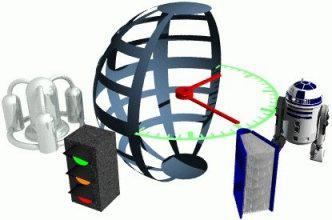
\includegraphics[]{img/test.jpg}
    \caption{Numele figurii}
    \label{fig:imag}
\end{figure}

Fiecare capitol 'incepe pe pagin'a nou'a.

\chapter{Obiectivele Proiectului}

'In acest capitol se prezint'a tema propriu-zis'a (sub forma unei teme de proiectare sau cercetare, formulat'a exact, cu obiective clare - 2-3 pagini 'si eventuale figuri explicative).

Reprezint'a cca. 10\% din lucrare.
\section{Titlu}
\section{Alt titlu}


\chapter{Studiu Bibliografic}

Documentarea bibliografic'a are ca obiectiv prezentarea stadiului actual al domeniului sau sub-domeniului 'in care se situeaz'a tema. 
'In redactarea acestui capitol ('in general a 'intregului document) se va 'tine cont de cuno'stin'tele acumulate la disciplinele dedicate din semestrul 2, anul 4 
(Metodologia 'Intocmirii Proiectelor, etc.), precum 'si la celelalte discipline relevante temei abordate.

Acest capitol reprezint'a cca. 15\% din lucrare.

Referin'tele se scriu 'in sec'tiunea Bibliografie. 
Formatul referin'telor trebuie s'a fie de tipul IEEE sau asem'an'ator. 
Introducerea 'si formatarea referin'telor 'in bibliografie, respectiv citarea 'in text, se pot face manual sau folosind instrumentele de lucru men'tionate 'in ultimele paragrafe din acest capitol.




In chapter~\ref{ch:analysis} of~\cite{strunk}, which discusses the value of the honeypots, Spitzner presents the advantages and disadvantages of such systems. 


'In sec'tiunea {\it Bibliografie} sunt exemple de referin'te pentru articol la conferin'te sau seminarii~\cite{BellucciLZ04}, articol 'in jurnal~\cite{AntoniouSBDB07}, 
sau c'ar'ti~\cite{russell1995artificial}. 


Referin'tele spre aplica'tii sau resurse online (pagini de internet) trebuie sa includ'a cel pu'tin o denumire sugestiv'a pe l\ia ng'a link-ul propriu-zis~\cite{webpage}, 
plus alte informa'tii dac'a sunt disponibile (autori, an, etc.). 
Referin'tele care prezint'a doar link spre resursa online se vor plasa 'in subsolul paginii unde sunt referite.
Citarea referin'telor 'in text este obligatorie, vezi exemplul de mai jos ('in func'tie de tema proiectului se poate varia modul de prezentare a metodei/aplica'tiei).

%'In articolul~\cite{AntoniouSBDB07} autorii prezint'a un sistem pentru ...
'In~\cite{AntoniouSBDB07} autorii prezint'a un sistem pentru detec'tia obstacolelor 'in mi'scare folosind stereoviziune 'si estimarea mi'sc'arii proprii. 
Metoda se bazeaz'a pe ...{\it trecere 'in revist'a a algoritmilor, structurilor de date, func'tionalitate, aspecte specifice temei proiectului etc}. Discu'tie {\it avantaje - dezavantaje}.


'In capitolul~\ref{ch:analysis} al~\cite{russell1995artificial} se prezint'a ...  


\section{Titlu}
\section{Alt titlu}


\chapter{Analiz'a 'si Fundamentare Teoretic'a}
\label{ch:analysis}

'Impreun'a cu capitolul urm'ator trebuie s'a reprezinte aproximativ 60\% din total.

Scopul acestui capitol este de a explica principiile func'tionale ale aplica'tiei implementate. 
Aici se va descrie solu'tia propus'a dintr-un punct de vedere teoretic - explica'ti 'si demonstra'ti propriet'a'tile 'si valoarea teoretic'a:
\begin{itemize}
 \item algoritm utilizat sau propus
\item protocoale utilizate
\item modele abstracte
\item explica'tii/argument'ari logice ale solu'tiei alese
\item structura logic'a 'si func'tional'a a aplica'tiei.
\end{itemize}

{\color{red}
NU SE FAC referiri la implementarea propriu-zis'a. 

NU SE PUN descrieri de tehnologii preluate cu copy-paste din alte surse sau lucruri care nu 'tin strict de proiectul propriu-zis (materiale de umplutur'a).
}


\section{Titlu}
\section{Alt titlu}


\chapter{Proiectare de Detaliu 'si Implementare}

'Impreun'a cu capitolul precedent reprezint'a aproximativ 60\% din total.

Scopul acestui capitol este de a documenta aplica'tia dezvoltat'a 'in a'sa fel 'inc\ia t dezvoltarea 'si 'intre'tinerea ulterioar'a s'a fie posibile. 
Cititorul trebuie s'a identifice func'tiile principale ale aplica'tiei din ceea ce este scris aici.
Capitolul ar trebui sa con'tin'a (nu se rezum'a neap'arat la):
\begin{itemize}
 \item schema general'a a aplica'tiei
\item descrierea fiec'arei componente implementate, la nivel de modul
\item diagrame de clase, clase importante 'si metode ale claselor importante.
\end{itemize}


\chapter{Testare 'si Validare}

Aproximativ 5\% din total

\section{Titlu}
\section{Alt titlu}

\chapter{Manual de Instalare 'si Utilizare}

'In sec'tiunea de Instalare trebuie s'a detalia'ti resursele software 'si hardware necesare pentru instalarea 'si rularea aplica'tiei, precum 'si o descriere pas cu pas a procesului de instalare. 
Instalarea aplica'tiei trebuie s'a fie posibil'a pe baza a ceea ce se scrie aici.

'In acest capitol trebuie s'a descrie'ti cum se utilizeaz'a aplica'tia din punct de vedere al utilizatorului, f'ar'a a men'tiona aspecte tehnice interne.
Folosi'ti capturi ale ecranului 'si explica'tii pas cu pas ale interac'tiunii. 
Folosind acest manual, o persoan'a ar trebui s'a poat'a utiliza produsul vostru.

\section{Titlu}
\section{Alt titlu}

\chapter{Concluzii}

Cca. 5\% din total.
Capitolul ar trebui sa con'tin'a (nu se rezum'a neap'arat la):
\begin{itemize}
 \item un rezumat al contribu'tiilor voastre
\item analiz'a critic'a a rezultatelor ob'tinute
\item descriere a posibilelor dezvolt'ari 'si 'imbun'at'a'tiri ulterioare
\end{itemize}


\section{Titlu}
\section{Alt titlu}


%\addcontentsline {toc}{chapter}{Bibliography} 
\bibliographystyle{IEEEtran} 
\bibliography{thesis}%same file name as for .bib

\appendix
\chapter{Relevant code}


\chapter{Other relevant information (demonstrations, etc.)}


\chapter{Published papers}

\end{document}
